 \let\negmedspace\undefined
\let\negthickspace\undefined
\documentclass[journal]{IEEEtran}
\usepackage[a5paper, margin=10mm, onecolumn]{geometry}
%\usepackage{lmodern} % Ensure lmodern is loaded for pdflatex
\usepackage{tfrupee} % Include tfrupee package

\setlength{\headheight}{1cm} % Set the height of the header box
\setlength{\headsep}{0mm}     % Set the distance between the header box and the top of the text

\usepackage{gvv-book}
\usepackage{gvv}
\usepackage{cite}
\usepackage{amsmath,amssymb,amsfonts,amsthm}
\usepackage{algorithmic}
\usepackage{graphicx}
\usepackage{textcomp}
\usepackage{xcolor}
\usepackage{txfonts}
\usepackage{listings}
\usepackage{enumitem}
\usepackage{mathtools}
\usepackage{gensymb}
\usepackage{comment}
\usepackage[breaklinks=true]{hyperref}
\usepackage{tkz-euclide} 
\usepackage{listings}
% \usepackage{gvv}                                        
\def\inputGnumericTable{}                                 
\usepackage[latin1]{inputenc}                                
\usepackage{color}                                            
\usepackage{array}                                            
\usepackage{longtable}                                       
\usepackage{calc}                                             
\usepackage{multirow}                                         
\usepackage{hhline}                                           
\usepackage{ifthen}                                           
\usepackage{lscape}
\begin{document}

\bibliographystyle{IEEEtran}
\vspace{3cm}

\title{10.4.ex-13.2}
\author{EE24BTECH11058 - P.Shiny Diavajna}
% \maketitle
% \newpage
% \bigskip
{\let\newpage\relax\maketitle}

\renewcommand{\thefigure}{\theenumi}
\renewcommand{\thetable}{\theenumi}
\setlength{\intextsep}{10pt} % Space between text and floats


\numberwithin{equation}{enumi}
\numberwithin{figure}{enumi}
\renewcommand{\thetable}{\theenumi}
\textbf{Question:} Solve the Quadratic equation 
\begin{align}
    x^2+4x+5=0
\end{align}

\textbf{Theoretical Solution:}\\
The roots of a Standard Quadratic equation of the form $ax^2+bx+c=0$ are given by the quadratic formula
\begin{align}
   x&=\frac{-b \pm \sqrt{b^2 - 4ac}}{2a}
\end{align}
Here, $a=1$,$b=4$ and $c=5$.On substituting the values in (0.2), we have 
\begin{align}
    x&= \frac{-4 \pm \sqrt{16-20}}{2}\\
    x&=-2 \pm i
\end{align}

\textbf{Computational Solution:}\\
Eigenvalues of Companion matrix:\\
The eigenvalues of a companion matrix are the roots of the characteristic polynomial that defines the matrix.
For a polynomial 
\begin{align}
    p(x)=x^n+a_{n-1}x^{n-1}+a_{n-2}x^{n-2}+ \dots +a_0
\end{align}Companion matrix A is defined as:
\begin{align}
    \myvec{0&1&0&\dots &0 \\0&0&1&\dots&0\\\vdots&\vdots&\vdots&\ddots&\vdots\\0&0&0&\dots&1\\-a_0 & -a_1 & -a_2 & \dots & -a_{n-1}}
\end{align}
Here, $a_0 =5$, $a_1=4$ 

\begin{align}
    A=\myvec{0 & 1\\-5 & -4}
\end{align}
We find the eigenvalues using the $QR$ algorithm. The basic principle behind this algorithm is a similarity transform,
\begin{align}
	A^{\prime} = X^{-1}AX
\end{align}
which does not alter the eigenvalues of the matrix A. 
\newline
We use this to get the Schur Decomposition,
\begin{align}
	A = Q^{-1}UQ = Q^{\ast}UQ
\end{align}
where $Q$ is a unitary matrix $\brak{Q^{-1} = Q^{\ast}}$ and $U$ is an upper triangular matrix whose diagonal entries are the eigenvalues of $A$.
\newline
To efficiently get the Schur Decomposition, we first householder reflections to reduce it to an upper hessenberg form.
\newline
A householder reflector matrix is of the form,
\begin{align}
	P = I - 2\vec{u}\vec{u^{\ast}}
\end{align}
Householder reflectors transforms any vector $\vec{x}$ to a multiple of $\vec{e_1}$,
\begin{align}
	P\vec{x} = \vec{x} - 2\vec{u}\brak{\vec{u^{\ast}}\vec{x}} = \alpha \vec{e_1}
\end{align}
P is unitary, which implies that,
\begin{align}
	\norm{P\vec{x}} &= \norm{\vec{x}}\\
	\implies \alpha &= \rho\norm{\vec{x}}\\
\end{align}
As $\vec{u}$ is unit norm,
\begin{align}
	\vec{u} = \frac{\vec{x} - \rho\norm{\vec{x}}\vec{e_1}}{\norm{\vec{x} - \rho\norm{\vec{x}}\vec{e_1}}} = \frac{1}{\norm{\vec{x} - \rho\norm{\vec{x}}\vec{e_1}}} \begin{pmatrix} x_1 - \rho\norm{\vec{x}}\\x_2\\\vdots\\x_n\end{pmatrix}
\end{align}
Selection of $\rho$ is flexible as long as $\abs{\rho} = 1$. To ease out the process, we take $\rho = \frac{x_1}{\abs{x_1}}$, $x_1 \neq 0$. If $x_1 = 0$, we take $\rho = 1$.
\newline
Householder reflector matrix $\brak{P_{i}}$ is given by,
\begin{align}
	P_{i} = 
	\begin{bmatrix}
		1 & 0 & 0 & 0 & 0\\    
		0 & \times & \times & \times & \times\\
		0 & \times & \times & \times & \times\\
		0 & \times & \times & \times & \times\\
		0 & \times & \times & \times & \times
	\end{bmatrix} = \begin{bmatrix}
		1 & \vec{0}^{\ast}\\    
		\vec{0} & I_{n - i} - 2\vec{u_{i}}\vec{u_{i}^{\ast}}
	\end{bmatrix}
\end{align}
\begin{align}
	\begin{bmatrix}
		\times & \times & \times & \times \\
		\times & \times & \times & \times \\
		\times & \times & \times & \times \\
		\times & \times & \times & \times
	\end{bmatrix}
	\xrightarrow{P_1}
	\begin{bmatrix}
		\times & \times & \times & \times \\
		\times & \times & \times & \times \\
		0 & \times & \times & \times \\
		0 & \times & \times & \times
	\end{bmatrix}
	\xrightarrow{P_2}
	\begin{bmatrix}
		\times & \times & \times & \times \\
		\times & \times & \times & \times \\
		0 & \times & \times & \times \\
		0 & 0 & \times & \times
	\end{bmatrix}
\end{align}
Next step is to do Given's rotation to get the $QR$ Decomposition.
\newline
The Givens rotation matrix $G\brak{i, j, c, s}$ is defined by
\begin{align}
	G\brak{i, j, c, s} = 
	\begin{bmatrix}
		1 & \cdots & 0 & \cdots & 0 & \cdots & 0 \\
		\vdots & \ddots & \vdots & \ddots & \vdots & \ddots & \vdots \\
		0 & \cdots & c & \cdots & s & \cdots & 0 \\
		\vdots & \ddots & \vdots & \ddots & \vdots & \ddots & \vdots \\
		0 & \cdots & -\overline{s} & \cdots & \overline{c} & \cdots & 0 \\
		\vdots & \ddots & \vdots & \ddots & \vdots & \ddots & \vdots \\
		0 & \cdots & 0 & \cdots & 0 & \cdots & 1
	\end{bmatrix}
\end{align}
where $\abs{c}^2 + \abs{s}^2 = 1$, and $G$ is a unitary matrix.
\newline
Say we take a vector $\vec{x}$, and $\vec{y} = G\brak{i, j, c, s}\vec{x}$, then
\begin{align}
	y_k = \begin{cases}
		c x_i + s x_j, & k = i \\
		-\overline{s} x_i + \overline{c} x_j, & k = j \\
		x_k, & k \neq i, j
	\end{cases}
\end{align}
For $y_j$ to be zero, we set
\begin{align}
	c = \frac{\overline{x_i}}{\sqrt{\abs{x_i}^2 + \abs{x_j}^2}} = c_{ij}\\
	s = \frac{\overline{x_j}}{\sqrt{\abs{x_i}^2 + \abs{x_j}^2}} = s_{ij}
\end{align}
Using this Givens rotation matrix, we zero out elements of subdiagonal in the hessenberg matrix $H$.
\begin{multline}
	H = \begin{bmatrix}
		\times & \times & \times & \times & \times\\
		\times & \times & \times & \times & \times\\
		0 & \times & \times & \times & \times\\
		0 & 0 & \times & \times & \times\\
		0 & 0 & 0 & \times & \times
	\end{bmatrix} \xrightarrow{G\brak{1, 2, c_{12}, s_{12}}}
	\begin{bmatrix}
		\times & \times & \times & \times & \times\\
		0 & \times & \times & \times & \times\\
		0 & \times & \times & \times & \times\\
		0 & 0 & \times & \times & \times\\
		0 & 0 & 0 & \times & \times
	\end{bmatrix} \\\xrightarrow{G\brak{2, 3, c_{23}, s_{23}}}
	\begin{bmatrix}
		\times & \times & \times & \times & \times\\
		0 & \times & \times & \times & \times\\
		0 & 0 & \times & \times & \times\\
		0 & 0 & \times & \times & \times\\
		0 & 0 & 0 & \times & \times
	\end{bmatrix} \xrightarrow{G\brak{3, 4, c_{34}, s_{34}}}
	\begin{bmatrix}
		\times & \times & \times & \times & \times\\
		0 & \times & \times & \times & \times\\
		0 & 0 & \times & \times & \times\\
		0 & 0 & 0 & \times & \times\\
		0 & 0 & 0 & \times & \times
	\end{bmatrix} \\\xrightarrow{G\brak{4, 5, c_{45}, s_{45}}}
	\begin{bmatrix}
		\times & \times & \times & \times & \times\\
		0 & \times & \times & \times & \times\\
		0 & 0 & \times & \times & \times\\
		0 & 0 & 0 & \times & \times\\
		0 & 0 & 0 & 0 & \times
	\end{bmatrix} = R
\end{multline}
where $R$ is upper triangular.
For the given companion matrix,

Let $G_k = G\brak{k, k + 1, c_{k, k+1}, s_{k, k+1}}$, then we deduce that
\begin{align}
	G_4 G_3 G_2 G_1 H &= R\\
	H &= G_1^{\ast} G_2^{\ast} G_3^{\ast} G_4^{\ast} R\\
	H &= QR, \text{ where } Q = G_1^{\ast} G_2^{\ast} G_3^{\ast} G_4^{\ast}
\end{align}
Using this $QR$ algorithm, we get the following update equation,
\begin{align}
	A_{k} &= Q_{k}R_{k}\\
	A_{k + 1} &= R_{k}Q_{k}\\
	&= \brak{G_{n}\dots G_{2} G_{1}} A_{k} \brak{G_1^{\ast} G_2^{\ast} \dots G_n^{\ast}}
\end{align}
Running the eigenvalue code we get
\begin{align}
	x_1 &=  -2.000000000000001 + -1.000000000000003j
\end{align}
\begin{align}
	x_2 &=  -2.000000000000001 + -1.000000000000003j
\end{align}
Newton-Raphson iterative method:
\begin{align}
    f\brak{x} &= x^2 + 4x +5
\end{align}
\begin{align}
    f^\prime\brak{x} &= 2x +4
\end{align}

Difference equation,
\begin{align}
    x_{n+1} &= x_n - \frac{f\brak{x_{n}}}{f^\prime\brak{x_n}}
\end{align}
\begin{align}
    x_{n+1} &= x_n - \frac{x_n^2 + 4x+5}{2x_n+4}
\end{align}
\begin{align}
    x_{n+1} &= \frac{x_n}{2} - 1-\frac{1}{2x_n +4}
\end{align}

Picking two initial guesses,
\begin{align}
     x_0&=0+i \text{ converges to } -2.0 + 1.0000000000000002i\\
     x_0&=0-i \text{ converges to } -2.0 + -1.0000000000000002i
\end{align}

\newpage
\textbf{Plot:}
\begin{figure}[h]
   \centering
   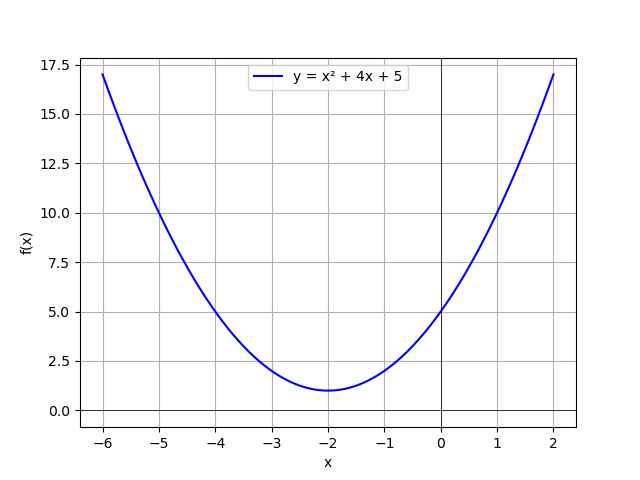
\includegraphics[width=\columnwidth]{figs/figure.png}
\end{figure}


Acknowledgments:\\  
Code from [https://github.com/Dwarak-A/sprog/tree/c6f873e29ab9910f22e49f7421dfc8e5fd5c60
fc/ncert/10/4/1/1/2/codes].
\end{document}    

